\documentclass[aspectratio=169,12pt,spanish]{beamer}
\usepackage[T1]{fontenc}
\usepackage[spanish]{babel}
\usepackage{wrapfig}
%\usepackage{siunitx}

\usepackage{multicol}
\usepackage{mathtools}

\usepackage[normalem]{ulem}

\pagestyle{empty}

\usepackage{pgf,tikz}
\usetikzlibrary{matrix}
\usetikzlibrary{arrows}

%\usepackage{wrapfig}
\mode<presentation>
\usefonttheme{professionalfonts}
\usetheme{Darmstadt}
\usecolortheme{orchid}
\useoutertheme{default}
\setbeamertemplate{headline}{}

\renewcommand{\baselinestretch}{1.1}

%gets rid of bottom navigation bars
\setbeamertemplate{footline}[page number]

%gets rid of navigation symbols
\setbeamertemplate{navigation symbols}{}

%\frameframe{none} % No default frame

%\setlength{\framewidth}{8.7in} \setlength{\frameheight}{7.2in}

\parindent 0pt
\setlength{\parskip} {1ex plus 0.5ex minus 0.2ex}


\usepackage[bbgreekl]{mathbbol}
\usepackage{amssymb, amsthm, amsmath}
\usepackage{bm}

\DeclareSymbolFontAlphabet{\mathbb}{AMSb}
\DeclareSymbolFontAlphabet{\mathbbl}{bbold}

\usepackage{multicol}
\usepackage{colortbl}
\usepackage{lmodern}
\usepackage{tabularx}
\usepackage{multirow}
\usepackage{stmaryrd}
\usepackage{color}
\usepackage{graphicx}
\graphicspath{ {../../images} }
\usepackage{hyperref}

\newtheorem{ejercicio}{Ejercicio}

\usepackage{listings}
\lstset{
  basicstyle=\ttfamily,
  columns=fullflexible,
}

\usepackage{url}
\usepackage{multicol}
\usepackage{dsfont}

% Bold symbols for vectors and matrices
\newcommand{\xstar}{\bm{x}^{\star}}
\newcommand{\alphab}{\bm{\alpha}}
\newcommand{\ab}{\bm{a}}
\newcommand{\bb}{\bm{b}}
\newcommand{\cb}{\bm{c}}
\newcommand{\db}{\bm{d}}
\newcommand{\eb}{\bm{e}}
\newcommand{\gb}{\bm{g}}
\newcommand{\mb}{\bm{m}}
\newcommand{\pb}{\bm{p}}
\newcommand{\qb}{\bm{q}}
\newcommand{\rb}{\bm{r}}
\newcommand{\ssb}{\bm{s}}
\newcommand{\ub}{\bm{u}}
\newcommand{\vb}{\bm{v}}
\newcommand{\wb}{\bm{w}}
\newcommand{\xb}{\bm{x}}
\newcommand{\yb}{\bm{y}}
\newcommand{\zb}{\bm{z}}

\newcommand{\Ab}{\bm{A}}
\newcommand{\Bb}{\bm{B}}
\newcommand{\Cb}{\bm{C}}
\newcommand{\Db}{\bm{D}}
\newcommand{\Eb}{\bm{E}}
\newcommand{\Fb}{\bm{F}}
\newcommand{\Gb}{\bm{G}}
\newcommand{\Hb}{\bm{H}}
\newcommand{\Ib}{\bm{I}}
\newcommand{\Id}{\bm{I}}
\newcommand{\Kb}{\bm{K}}
\newcommand{\Lb}{\bm{L}}
\newcommand{\Mb}{\bm{M}}
\newcommand{\Pb}{\bm{P}}
\newcommand{\Qb}{\bm{Q}}
\newcommand{\Rb}{\bm{R}}
\newcommand{\Sb}{\bm{S}}
\newcommand{\Tb}{\bm{T}}
\newcommand{\Ub}{\bm{U}}
\newcommand{\Vb}{\bm{V}}
\newcommand{\Wb}{\bm{W}}
\newcommand{\Xb}{\bm{X}}
\newcommand{\Yb}{\bm{Y}}
\newcommand{\Zb}{\bm{Z}}
\newcommand{\Lambdab}{\bm{\Lambda}}
\newcommand{\cero}{\bm{0}}

% Rings and fields
\newcommand{\A}{\mathbb{A}}
\newcommand{\Z}{\mathbb{Z}}
\newcommand{\Q}{\mathbb{Q}}
\newcommand{\C}{\mathbb{C}}
\newcommand{\R}{\mathbb{R}}
\newcommand{\K}{\mathbb{K}}
\newcommand{\N}{\mathbb{N}}

\newcommand{\borel}{{\mathcal B}}
\newcommand{\pmom}{{\rho_{\text{mom}}}}
\newcommand{\MX}{{\mathcal{M}(X)}}


% Inner product
\newcommand{\innerl}[2]{\langle #1, #2 \rangle}
\newcommand{\inner}[2]{#1 \boldsymbol{\cdot} #2}
\newcommand{\innerTrace}[2]{#1 \bullet #2}

% Symmetric and positive definite matrices
\newcommand{\Splusplusn}{{\mathcal S_{++}^n}}
\newcommand{\Splusn}{{\mathcal S_+^n}}
\newcommand{\Splus}{{\mathcal S_+}}
\newcommand{\Sym}{{\mathcal S}}
\newcommand{\Symn}{{\mathcal S^n}}

% Cones
\newcommand\CC{\mathcal{C}}
\DeclareMathOperator{\cone}{cono}
\DeclareMathOperator{\conv}{conv}
\DeclareMathOperator{\supp}{supp}


% Spectrahedron
\newcommand{\eLL}{{\mathcal L}}

% Matrices and vectors over R or C
\newcommand{\Rnn}{\R^{n\times n}}
\newcommand{\Cnn}{\C^{n\times n}}
\newcommand{\Rn}{\R^{n}}
\newcommand{\Rm}{\R^{m}}


% Math operators
\DeclareMathOperator{\Tr}{Tr}
\DeclareMathOperator{\tr}{Tr}
\DeclareMathOperator{\interior}{int}
\DeclareMathOperator{\rank}{rank}
\DeclareMathOperator{\diag}{diag}

\newcommand\one{\mathds{1}} 


\newcommand{\ideal}[1]{{\left\langle{#1}\right\rangle}}
\newcommand{\demo}{\textbf {Demostraci\'on. }}
\newcommand{\obse}{\textbf {Observaci\'on. }}
\newcommand{\Input}{\textbf {Input: }}
\newcommand{\Output}{\textbf {Output: }}
\newcommand{\Examp}{\textbf {Ejemplo }}
\newcommand{\Examps}{\textbf {Ejemplos }}

\begin{document}

\begin{frame}

\begin{center}

\Large\textbf{Optimización Semidefinida} \\
\large\textbf{Introducción}
%\vspace{0.5cm}

% \textit{Santiago Laplagne} \\
%slaplagn@dm.uba.ar \\


%\vspace{0.5cm}
%{\small Trabajo en progreso en conjunto con \emph{Jose Capco} (Universit\"at Innsbruck) y \emph{Claus Scheiderer} %(Universit\"at Konstanz).} \\

\vspace{1cm}
 Segundo Cuatrimestre 2021
 \\
 {\small Facultad de Ciencias Exactas y Naturales, UBA}
 \end{center}

\end{frame}

%------------------------------------------------------------------

\begin{frame}
\frametitle{Organización de la materia}

\begin{itemize}
\item Régimen de aprobación
\item Inscripción en el SIU Guaraní
\item Puntaje para licenciatura y doctorado
\item Licencias de Mosek
\end{itemize}

\end{frame}

%------------------------------------------------------------------

\begin{frame}
\frametitle{Introducción: programación lineal}

Programaci\'on lineal es el problema de minimizar o maximizar una funci\'on lineal sujeta a restricciones lineales.

\textbf{Ejemplo.} Queremos maximizar la función
$$f(x_1, x_2) = 4x_1 + 6x_2$$
sujeta a las restricciones
\begin{alignat*}{2}
   & \quad & -x_1 + x_2 &\le 11,\\
   &   \quad & x_1 + x_2 &\le 27, \\
   &   \quad & 2x_1 + 5x_2 &\le 90, \\
   & &  x_1, x_2 &\ge 0.
\end{alignat*}

\end{frame}

%------------------------------------------------------------------

\begin{frame}
\frametitle{Introducción: programación lineal}

Cada una de las desigualdades en las restricciones define un semiplano en $\R^2$.
Podemos graficar el conjunto de todos los puntos de $\R^2$ que cumplen todas las restricciones intersecando los semiplanos correspondientes.

\begin{center}
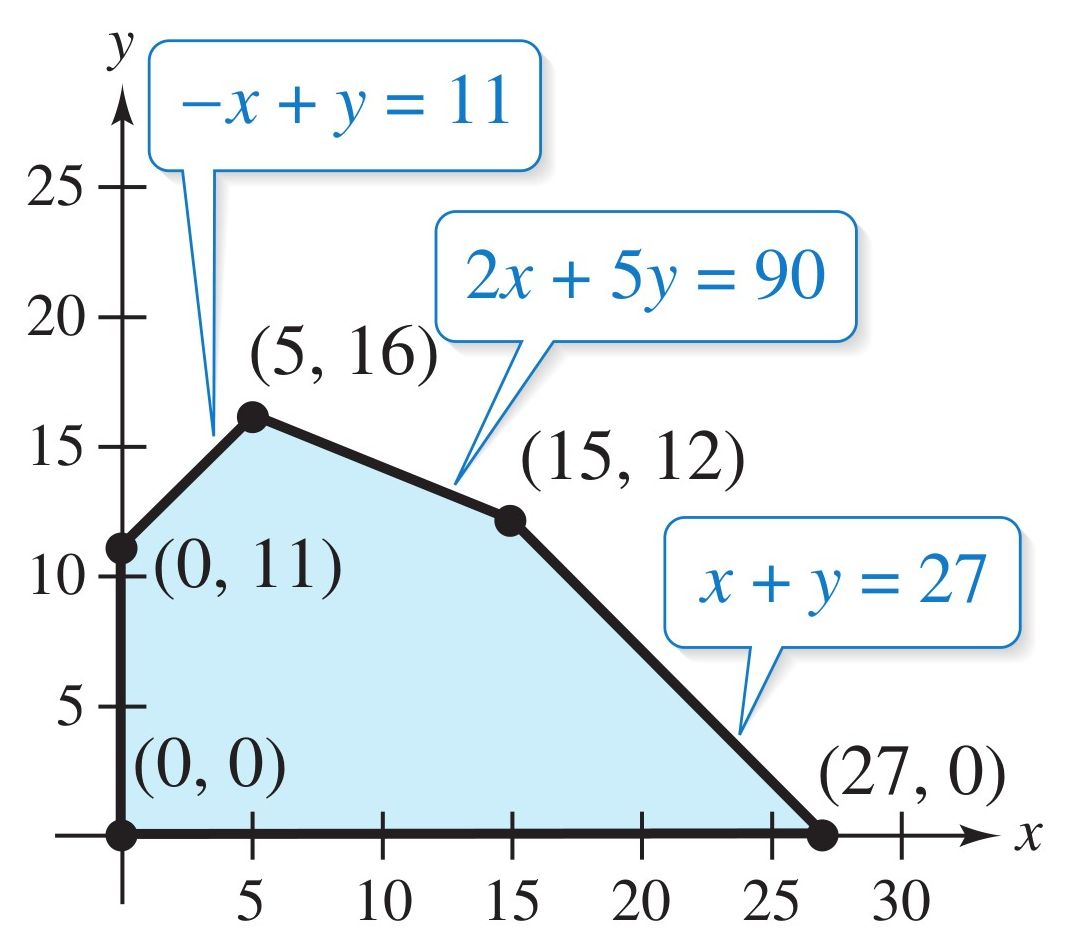
\includegraphics[scale=.2]{LP_ecuaciones.png}
\end{center}

\end{frame}

%------------------------------------------------------------------

\begin{frame}
\frametitle{Introducción: programación lineal}

El conjunto de puntos del plano para los cuales la función toma un valor fijo $z_0$ es una recta
$$
l(z_0) = \{(x_1, x_2) : 4x_1 + 6x_2 = z_0\}.
$$

Por ejemplo, si tomamos $z_0 = 120$ obtenemos la recta verde.

\begin{center}
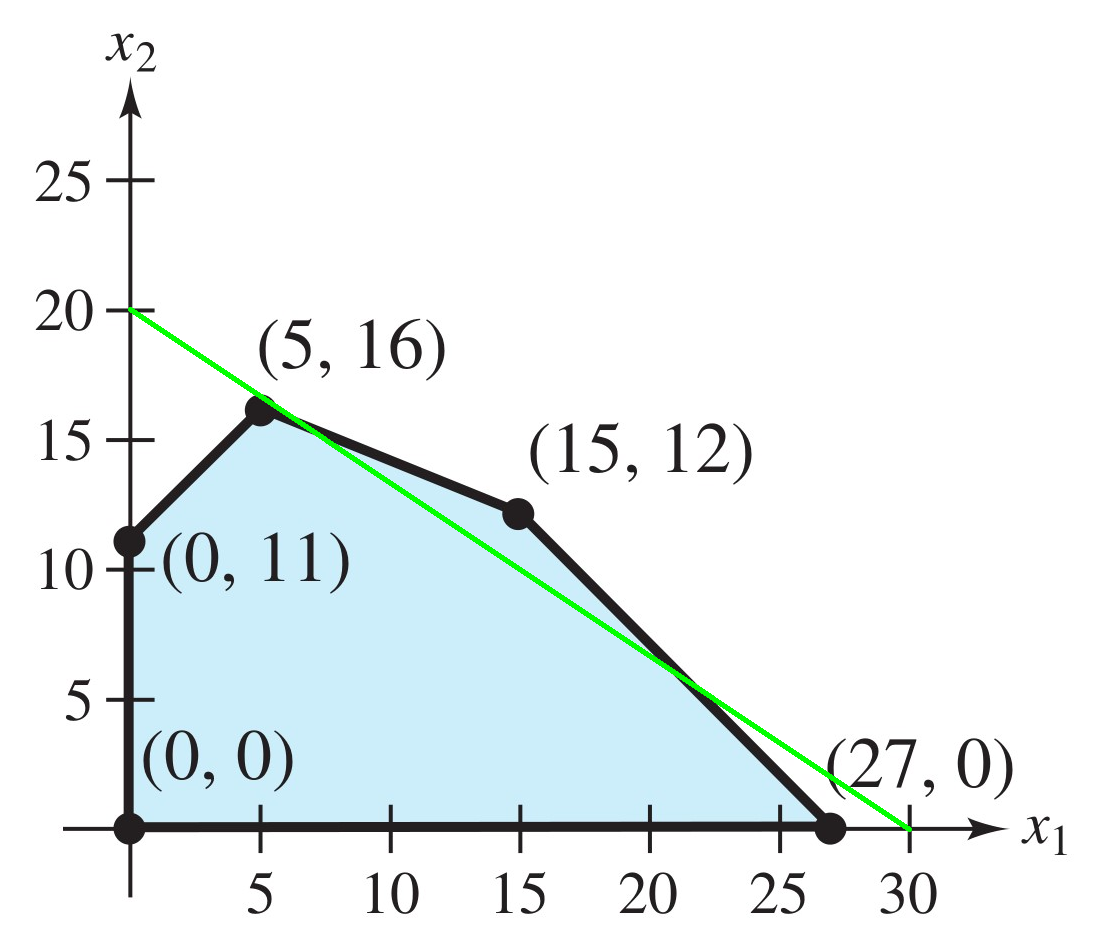
\includegraphics[scale=.2]{LP_line.png}
\end{center}

\end{frame}

%------------------------------------------------------------------

\begin{frame}
\frametitle{Introducción: programación lineal}

Geométricamente, si variamos el valor de $z_0$, estamos desplazando la recta obteniendo siempre rectas paralelas.

En nuestro ejemplo, si desplazamos la recta hacia arriba, el valor de $z_0$ aumenta, mientras que si desplazamos la recta hacia abajo, el valor de $z_0$ disminuye.

\begin{minipage}{0.6\textwidth}
Podemos resolver el problema gráficamente, desplazando la recta hacia arriba todo lo que podamos mientras que la intersección de la recta con la figura sea no vacía.

El máximo es $4 \times 15 + 6 \times 12 = 132$.
\end{minipage}
\begin{minipage}{0.35\textwidth}
\begin{center}
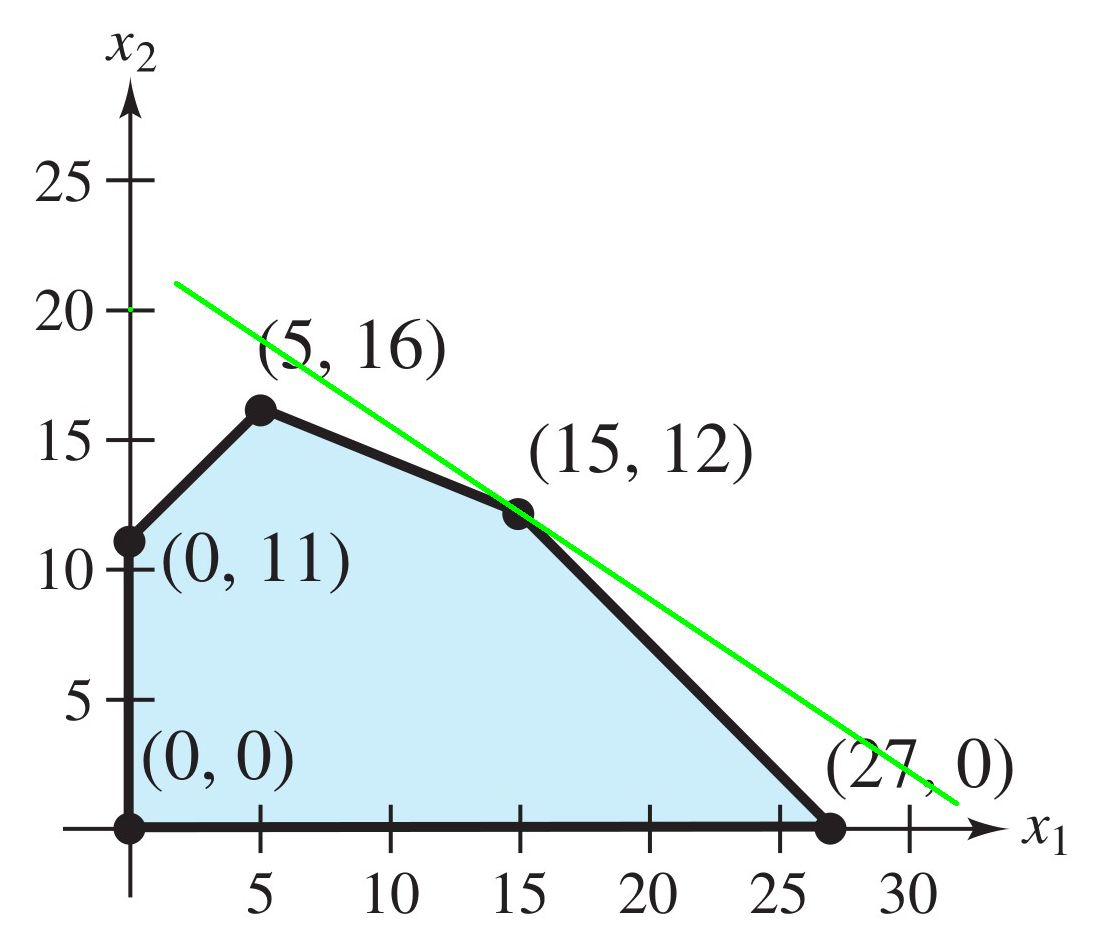
\includegraphics[scale=.15]{LP_line_parallel.png}
\end{center}
\end{minipage}



\end{frame}

%------------------------------------------------------------------

\begin{frame}
\frametitle{Introducción: programación lineal}

Mediante esta resolución gráfica, podemos observar algunas propiedades del problema de programación lineal.

\begin{itemize}
\item Si la región de puntos que satisfacen las restricciones es acotada, forma un polígono, y el óptimo de la función a optimizar se alcanza en el borde del polígono.
\item Más precisamente en un vértice del polígono (puede suceder que el óptimo se alcance también sobre todo un lado del polígono).
\item En particular, dado que un polígono tiene una cantidad finita de vértices, el problema de programación lineal puede resolverse algorítmicamente evaluando la función objetivo sobre todos los vértices del polígono.
\end{itemize}

\end{frame}

%------------------------------------------------------------------

\begin{frame}
\frametitle{Introducción: programación semidefinida}

\textbf{Ejemplo.} Dado el polinomio  $f(x) = 10x^4+2x^3+27x^2-24x+5$, queremos determinar si $f(x) \ge 0$ para todo $x \in \R$.

\textbf{Propiedad.} Un polinomio $f \in \R[x]$ de grado $2d$ es no-negativo para todo $x \in \R$ si y solo si $f$ se puede escribir como una suma de cuadrados
$$
f = p_1^2 + p_2^2 +  \dots + p_s^2,
$$
con polinomios $p_i \in \R[x]$ de grado $\le d$, $1 \le i \le s$.

Podemos escribir esta igualdad matricialmente:
$$
f =  \begin{pmatrix}
p_1 & p_2 & \cdots & p_s \end{pmatrix}
\begin{pmatrix}
p_1 \\ p_2 \\ \vdots \\ p_s
\end{pmatrix}
=  \begin{pmatrix}
p_1 & p_2 & \cdots & p_s \end{pmatrix}
\begin{pmatrix} 1 & & 0 \\ & \ddots & \\ 0 & & 1 \end{pmatrix}
\begin{pmatrix}
p_1 \\ p_2 \\ \vdots \\ p_s
\end{pmatrix}.
$$

\end{frame}

%------------------------------------------------------------------

\begin{frame}
\frametitle{Introducción: programación semidefinida}

Como cada $p_i \in \R[x]_d$,
$$p_i = \sum_{j=0}^d c_{ij} x^j$$
y obtenemos
$$
\begin{pmatrix}
p_1 \\ p_2 \\ \vdots \\ p_s
\end{pmatrix} =
\begin{pmatrix} c_{10} & c_{11} & \dots & c_{1d} \\
c_{20} & c_{21} & \dots & c_{2d} \\
& & \ddots & \\ c_{s0} & c_{s1} & & c_{sd} \end{pmatrix}
\begin{pmatrix}
1 \\ x \\ \vdots \\ x^d
\end{pmatrix}.
$$

\end{frame}

%------------------------------------------------------------------

\begin{frame}
\frametitle{Introducción: programación semidefinida}

Concluimos que podemos escribir a $f$ como
$$
f = \begin{pmatrix}
1 & x & x^2 & \dots & x^d
\end{pmatrix}
\Cb^T \Cb
\begin{pmatrix}
1 \\ x \\ \vdots \\ x^d
\end{pmatrix},
$$
donde $\Cb \in \R^{s \times (d+1)}$ y $\Cb^T \Cb \in \R^{(d+1) \times (d+1)}$ es una matriz semidefinida positiva.

Recíprocamente, si $f(x) = \vb^T \Qb \vb$, con $\vb$ el vector de monomios y $\Qb \in \R^{(d+1) \times (d+1)}$ semidefinida positiva, existe $\Cb$ tal que $\Qb = \Cb^T \Cb$ y podemos obtener una descomposición como suma de cuadrados.

\end{frame}

%------------------------------------------------------------------

\begin{frame}
\frametitle{Introducción: programación semidefinida}

Volviendo al ejemplo, planteamos la ecuación:
$$10x^4+2x^3+27x^2-24x+5 =
\begin{pmatrix}
1 & x & x^2
\end{pmatrix}
\begin{pmatrix}
a_{11} & a_{12} & a_{13} \\
a_{12} & a_{22} & a_{23} \\
a_{13} & a_{23} & a_{33} \\
\end{pmatrix}
\begin{pmatrix}
1 \\
x \\
x^2 \\
\end{pmatrix}
$$

Para determinar si $f \ge 0$ para todo $x \in \R$ tenemos que determinar si existe $\Ab \in \R^{3 \times 3}$ tal que
\begin{align*}
&a_{11} = 5, \quad 2a_{12} = -24, \quad 2a_{13} + a_{22} = 27, \quad 2a_{23} = 2, \quad a_{33} = 10, \\
&\Ab \succeq 0
\end{align*}


\end{frame}

%------------------------------------------------------------------


\begin{frame}
\frametitle{Introducción: programación semidefinida}

Observamos que las primeras restricciones son ecuaciones lineales en los coeficientes de la matriz incógnita. En general podemos plantear un problema de programación semidefinida en la forma
\begin{alignat*}{2}
  & \text{minimizar: }& \quad & \sum_{1\le i,j \le n} c_{ij} x_{ij} \\
  & \text{sujeto a: } & \quad & \sum_{1\le i,j \le n} a_{ij}^{(1)} x_{ij} = b^{(1)}, \dots, \sum_{1\le i,j \le n} a_{ij}^{(s)} x_{ij} = b^{(s)}\\
   && & \Xb\succeq 0,
\end{alignat*}
donde $\Cb, \Ab_i$ ($1 \le i \le m$) son matrices simétricas y la matrix simétrica $\Xb$ es la variable sobre la cual realizamos la minimización.

\end{frame}

%------------------------------------------------------------------

\begin{frame}
\frametitle{Hiperplanos y semiespacios}

Dados vectores $\xb, \yb \in \R^n$, definimos $\inner{\xb}{\yb} = \sum_{i=1}^n x_i y_i$ el producto interno usual de $\R^n$.

\begin{definition}
Dado un vector no-nulo $\ab \in \R^n$ y un escalar $b$,
  \begin{enumerate}
  \item el conjunto $\{\xb \in \R^n | \inner{\ab}{\xb} = b\}$ es un \emph{hiperplano},
  \item el conjunto $\{\xb \in \R^n | \inner{\ab}{\xb} \le b\}$ es un \emph{semiespacio}.
  \end{enumerate}
\end{definition}

Dada una matriz $\Ab \in \R^{m \times n}$ y un vector $\bb \in \R^n$, en la condición $\Ab \xb = \bb$, cada fila $\ab_i$ de $\Ab$ impone la restricción $\inner{\ab_i}{\xb} = b_i$. 

El conjunto $\{\xb \in \R^n | \Ab \xb = \bb\}$ corresponde por lo tanto a una intersección de hiperplanos, que llamamos \emph{espacio afín}.

El conjunto $\{\xb \in \R^n | \Ab \xb \ge \bb\}$ corresponde a una intersección de semiespacios.

%Dada una matriz $\Ab \in \R^{m \times n}$ y un vector $\bb \in \R^n$, el conjunto $\{\xb \in \R^n | \Ab \xb = \bb\}$ corresponde a una intersección de hiperplanos, que llamamos \emph{espacio afín}. El conjunto $\{\xb \in \R^n | \Ab \xb \le \bb\}$ corresponde a una intersección de semiespacios.

\end{frame}

%------------------------------------------------------------------

\begin{frame}
\frametitle{Poliedros y polítopos}

Llamamos \emph{poliedro} a un conjunto definido por ecuaciones e inecuaciones lineales,
$$
P = \{\xb \in \R^n \mid \Ab_1 \xb = \bb_1, \Ab_2 \xb \ge \bb_2\}.
$$

En el caso de que el conjunto resulte acotado, lo llamamos \emph{pol\'itopo}.

Según nuestra definición, un poliedro no  necesariamente es un conjunto acotado.

\begin{center}
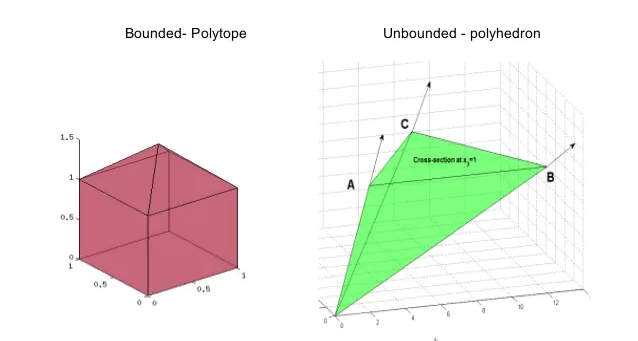
\includegraphics[scale=1.5]{polyhedron.png}
\end{center}

\end{frame}

%------------------------------------------------------------------

\begin{frame}
\frametitle{Conjuntos convexos}

\begin{definition}
Un conjunto $S \subset \R^n$ es convexo si para todos $\xb, \yb \in S$, el segmento con vértices $\xb$ e $\yb$ está incluido en $S$. Es decir, para todo $\lambda \in [0, 1]$,
$$
\lambda \xb + (1-\lambda) \yb \in S.
$$
\end{definition}

El punto $\zb = \lambda \xb + (1-\lambda) \yb$, $\lambda \in [0, 1]$, es una \emph{combinación convexa} de $\xb$ y $\yb$.

\begin{center}
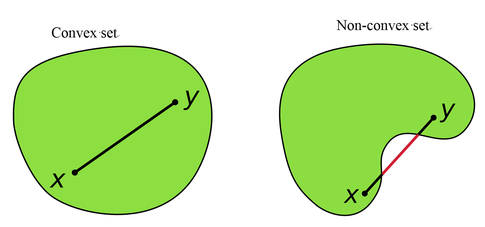
\includegraphics[scale=.25]{convexSet.png}
\end{center}


\textbf{Propiedad:} La intersección de dos conjuntos convexos es un conjunto convexo.


\end{frame}

%------------------------------------------------------------------

\begin{frame}
\frametitle{El problema de programación lineal}

Consideramos el problema de programación lineal
\begin{alignat*}{2}
  & \text{minimizar: } & & \inner{\cb}{\xb} \\
   & \text{sujeto a: } & \quad & \Ab\xb = \bb \\
   & & & \xb \ge \cero.
\end{alignat*}

Podemos interpretar geom\'etricamente el conjunto factible (\emph{feasible set} en ingl\'es), es decir la regi\'on sobre la que queremos minimizar $\inner{\cb}{\xb}$, como la intersecci\'on de un espacio af\'in (definido por la ecuaci\'on $\Ab\xb = \bb$) y el ortante positivo $\xb \ge \cero$.

El conjunto factible es un poliedro (en particular es un conjunto convexo).

\end{frame}

%------------------------------------------------------------------

\begin{frame}
\frametitle{El problema de programación lineal}

Una función $f: \R^n \rightarrow \R$,
$$f(\xb) = \inner{\cb}{\xb} = c_1 x_1 + \dots + c_n x_n,$$
$\cb \in \R^n$, la llamamos \emph{funcional lineal}.

\begin{block}{}
El problema de programación lineal consiste en optimizar una funcional lineal sobre un poliedro.
\end{block}


\end{frame}

%------------------------------------------------------------------

\begin{frame}
\frametitle{Programación Lineal}

\begin{ejercicio}
Dado el problema
\begin{alignat*}{2}
  & \text{minimizar: } & & 3 x_1 + 5 x_2 \\
   & \text{sujeto a: } & \quad & x_1 + x_2 = 6 \\
   & & & \xb \ge 0,
\end{alignat*}
graficar el conjunto factible, y resolver el problema.
\end{ejercicio}

\end{frame}

%------------------------------------------------------------------
\begin{frame}
\frametitle{Variables de holgura}

Dado el problema de programación lineal
\begin{alignat*}{2}
  & \text{minimizar: } & & \inner{\cb}{\xb} \\
   & \text{sujeto a: } & \quad & \Ab\xb \le \bb \\
   & & & \xb \ge \cero,
\end{alignat*}
cada fila $\ab_i$ de $\Ab$ impone una restricción $\inner{\ab_i}{\xb} \le b_i$.

Podemos convertir el problema en un problema con restricciones de igualdad reemplazando cada desigualdad $\inner{\ab_i}{\xb} \le b_i$ por las restricciones
$$\inner{\ab_i}{\xb} + s_i =  b_i, \quad \quad s_i \ge 0,$$
donde $s_i$ es una nueva variable del problema. Estas nuevas variables se llaman variables de holgura.

\end{frame}

%------------------------------------------------------------------
\begin{frame}
\frametitle{Variables de holgura}

Obtenemos el problema equivalente con restricciones de igualdad
\begin{alignat*}{2}
  & \text{minimizar: } & & \inner{\cb}{\xb} \\
   & \text{sujeto a: } & \quad & \inner{\ab_1}{\xb} + s_1 = b_1 \\
   &  & \quad & \dots \\
   &  & \quad & \inner{\ab_m}{\xb} + s_m = b_m \\
   & & & \xb \ge \cero, \ssb \ge \cero,
\end{alignat*}
con $\ssb = (s_1, \dots, s_m)$.

\end{frame}

%------------------------------------------------------------------
\begin{frame}
\frametitle{Variables de holgura}

\begin{ejercicio}
Dado el problema
\begin{alignat*}{2}
  & \text{minimizar: } & & 3 x_1 + 5 x_2 \\
   & \text{sujeto a: } & \quad & x_1 \le 1, x_2 \le 1 \\
   & & & \xb \ge 0,
\end{alignat*}
\begin{enumerate}
\item graficar el conjunto factible,
\item convertirlo a un problema con igualdades agregando las variables de holgura necesarias,
\item calcular las coordenadas de los vértices del poliedro en el nuevo problema.
\end{enumerate}
\end{ejercicio}

\end{frame}


\end{document}
